
\documentclass[11pt,letterpaper]{article}

%\usepackage{epsf}
%\usepackage{bib}
%\usepackage{floatflt}
\usepackage{cite}
\usepackage{subfigure}
%\usepackage{psfig}
\usepackage{pstricks}
\usepackage{fullpage}
\usepackage{amsthm}
\usepackage{graphics}
\usepackage{epsfig}
\usepackage{comment}
\usepackage[small,compact]{titlesec}
\usepackage[small,it]{caption}
%\usepackage[it]{caption}
%\usepackage{times}
\usepackage{wrapfig}
%\usepackage{nsf}
%%%%%%%%%%%%%%%%%%%%%%%%%%%%%%%%%%%%%%%%%%%%%%%%%%%%%%%%%%%%%%%%%%%%%%%%%
\pagestyle{plain}                                                      %%
%%%%%%%%%% EXACT 1in MARGINS %%%%%%%                                   %%
\setlength{\textwidth}{6.5in}     %%                                   %%
\setlength{\oddsidemargin}{0in}   %% (It is recommended that you       %%
\setlength{\evensidemargin}{0in}  %%  not change these parameters,     %%
%\setlength{\textheight}{8.5in}   %%  at the risk of having your       %%
\setlength{\textheight}{9.0in}    %%
\setlength{\topmargin}{0in}       %%  proposal dismissed on the basis  %%
\setlength{\headheight}{0in}      %%  of incorrect formatting!!!)      %%
\setlength{\headsep}{0in}         %%                                   %%
\setlength{\footskip}{.5in}       %%                                   %%
%%%%%%%%%%%%%%%%%%%%%%%%%%%%%%%%%%%%                                   %%
%\newcommand{\required}[1]{\section*{\hfil #1\hfil}}                    %%
%\renewcommand{\refname}{\hfil References Cited\hfil}                   %%
%\bibliographystyle{plain}                                              %%
%%%%%%%%%%%%%%%%%%%%%%%%%%%%%%%%%%%%%%%%%%%%%%%%%%%%%%%%%%%%%%%%%%%%%%%%%
\newcommand{\squishlist}{
   \begin{list}{$\bullet$}
    { \setlength{\itemsep}{0pt}      \setlength{\parsep}{0pt}
      \setlength{\topsep}{3pt}       \setlength{\partopsep}{0pt}
      \setlength{\listparindent}{-2pt}
      \setlength{\itemindent}{-5pt}
      %\setlength{\itemindent}{10pt}
      \setlength{\leftmargin}{1em} \setlength{\labelwidth}{0em}
      \setlength{\labelsep}{0.5em} } }

\newcommand{\squishlistindent}{
   \begin{list}{$\bullet$}
    { \setlength{\itemsep}{0pt}      \setlength{\parsep}{0pt}
      \setlength{\topsep}{3pt}       \setlength{\partopsep}{0pt}
      \setlength{\listparindent}{-2pt}
      %\setlength{\itemindent}{-5pt}
      \setlength{\itemindent}{20pt}
      \setlength{\leftmargin}{1em} \setlength{\labelwidth}{0em}
      \setlength{\labelsep}{0.5em} } }

\newcommand{\squishend}{
    \end{list}  }





\begin{document}


\vspace*{-0.5\baselineskip} \vspace*{-\baselineskip}
%\newpage

\thispagestyle{empty}

%

\documentclass[11pt,letterpaper]{article}

\usepackage{fullpage}
\usepackage{amsthm}
\usepackage{graphics}
\usepackage{epsfig}
\usepackage{comment}
\usepackage[small,compact]{titlesec}
\usepackage[small,it]{caption}
\usepackage{times}
 %\usepackage{nsf}
%%%%%%%%%%%%%%%%%%%%%%%%%%%%%%%%%%%%%%%%%%%%%%%%%%%%%%%%%%%%%%%%%%%%%%%%%
\pagestyle{plain}
%%
%%%%%%%%%% EXACT 1in MARGINS %%%%%%%                                   %%
\setlength{\textwidth}{6.5in}     %%                                   %%
\setlength{\oddsidemargin}{0in}   %% (It is recommended that you       %%
\setlength{\evensidemargin}{0in}  %%  not change these parameters,     %%
%\setlength{\textheight}{8.5in}   %%  at the risk of having your       %%
\setlength{\textheight}{9.0in}    %%
\setlength{\topmargin}{0in}       %%  proposal dismissed on the basis  %%
\setlength{\headheight}{0in}      %%  of incorrect formatting!!!)      %%
\setlength{\headsep}{0in}         %%                                   %%
\setlength{\footskip}{.5in}       %%                                   %%
%%%%%%%%%%%%%%%%%%%%%%%%%%%%%%%%%%%%                                   %%
%\newcommand{\required}[1]{\section*{\hfil #1\hfil}}                    %%
%\renewcommand{\refname}{\hfil References Cited\hfil}                   %%
%\bibliographystyle{plain}                                              %%
%%%%%%%%%%%%%%%%%%%%%%%%%%%%%%%%%%%%%%%%%%%%%%%%%%%%%%%%%%%%%%%%%%%%%%%%%

\begin{document}
\begin{center}
{\Large Collaborative Research: Design Methodologies and Circuit Techniques for Emerging Non-Volatile Memories}\\
\end{center}
\begin{center}
{\large  PROJECT SUMMARY} \\
%{Hai Li (NYU-Poly) and Yuan Xie (Penn State)}
\end{center}

\normalsize
%One of the major benefits that nanoscale technology offers is high density. Part of this density is deployed by high density memory technologies, including SRAM, DRAM, Flash memory, and hard disk drive. However, as device feature size continues scaling down to 32nm and below, these 
As technology scales, traditional memory technologies, such as SRAM and DRAM memories, are increasingly constrained by fundamental limits. Emerging non-volatile memory (NVM) technologies, such as \textit{Phase-change RAM (PCRAM)}, \textit{Magnetic RAM (MRAM)},  \textit{Resistive RAM (RRAM)}, and \textit{Memristor} are being explored as potential alternatives of existing memories in future computing systems. Such NVM technologies combine the speed of SRAM, the density of DRAM, and the non-volatility of Flash memory, and hence, become very attractive as the future universal memories. 

As such emerging memory technologies are getting mature, it is important for circuit designers to understand their pros and cons, refine and/or create new design techniques, and optimally exploit them to significantly improve the performance/power/reliability. \textit{The main objective of this project is to offer design methodologies and circuit design techniques for future emerging memory technologies, and to study the design implications of the emerging NVM technologies on future computer systems.}

%\vspace*{-2mm} 
{\flushleft{\bf Intellectual Merit}}: 
To explore new design opportunities that these emerging memory technologies can bring to the designers,  this project involves two research tasks including \emph{design methodologies and circuit techniques}, to study the implication of such NVM technologies for future computing system designs: (1) We propose to study the \textit{device modeling} and \textit{design methodologies} for emerging NVMs, and develop memory array design flow and optimization methodologies to facilitate the design space explorations; (2) We propose \textit{circuit techniques} to improve the reliability (including lifetime improvement and variation mitigation), yield,
and density for emerging memory technologies. The proposed research takes a holistic design perspective with close collaboration between two PIs with complementary expertise, and with close partnerships with industry collaborators, aiming at accelerating the adoption of emerging NVMs for future VLSI circuit design.

The key \textit{\textbf{transformative aspect}} of the proposed research is that, the success of the project will result in innovations in memory design techniques, accelerating the commercialization of the emerging NVM technologies, and potentially leading to better performance, higher energy-efficient, and more reliable computer systems.

%\vspace*{-2mm} 
{\flushleft{\bf Broader Impacts}}: The research will be be conducted in collaboration with our industrial partners, including HP, IBM, Intel, Seagate, Qualcomm, as well as IMEC. Through close collaboration with several industry partners, we envision direct transfer of many ideas to industry. The outcome of this research will, therefore, have a direct impact on future computer system. Undergraduate and graduate students involved in this research will get versatile training in several areas to prepare them for the next-generation IT workforce. We will actively seek under-represented students to participate in this project. We plan to develop a new graduate-level course on emerging non-volatile memories offered simultaneously at Penn State and NYU-Poly. The course will provide students a spectrum of inter-related issues from technology, device, to circuit and architectures. The design methodologies and circuit techniques developed in this research will be used in developing this new course. Finally, the device models and design flow developed in this research will be made available through our web-sites for use by other educators, researchers, and industry practitioners. We will also organize tutorials along with major conferences to disseminate the results from this work.

\paragraph{\textbf{Key Words:}} non-volatile memories; memory design; memory modeling and analysis; design methodology; emerging technology

\end{document}
%\normalsize

%\newpage
\setcounter{page}{1}

\begin{center}
{\Large Device and Circuit Techniques for Emerging Non-Volatile Memories}\\
% in Hybrid Computing Systems
\vspace*{0.75\baselineskip}
{\Large Project Description}\\

\end{center}

\section{Objective and Significance}

The traditional memory technologies, e.g. SRAM, DRAM, and Flash memory, played a very important role in the modern computing system and portable multimedia device industries. However, the scaling of the traditional memories is facing significant challenges from process variations and device reliability at 22nm technology and below~\cite{ITRS07,Kinam07}.
In recent years, significant efforts and resources have been put on the researches and developments of \textbf{emerging non-volatile memory (NVM) technologies} that combine attractive features such as scalability, fast read/write, negligible leakage, and non-volatility. Multiple promising candidates, such as \emph{Phase-Change RAM (PCRAM)}, \emph{Magnetic RAM (MRAM)}, \emph{Resistive RAM (RRAM)} and \emph{Memristor}, have gained substantial attentions and are being actively pursued by industry~\cite{ITRS07,burr:scm08}.

The main objective of this 3-year project is to investigate design methodologies and circuit techniques for emerging NVMs in order to enable the massive production and to accelerate the commercialization of these emerging memory technologies. The proposed program makes the following major contributions.

\vspace{5pt}
\squishlist
\item {\textbf{Design methodologies for emerging NVMs:} The device models for emerging NVMs will be built to fill the gap between process development and circuit design. Memory design flow and optimization methodologies will be developed to facilitate the design space explorations.}
\item {\textbf{Circuit techniques for emerging NVM technologies:} Various circuit techniques will be proposed to improve the reliability (including lifetime improvement and variation mitigation), yield, and density.}
\item {\textbf{Integrated educational plan:} The educational plan will enhance the existing standard curricula by integrating new course modules on emerging NVMs to complement and upgrade the core device and circuit design courses, and bring the awareness of emerging memory technologies into the circuit design and computer architecture community through tutorials and workshops.}
\squishend
\vspace{5pt}

The proposed work will initiate a novel research direction in memory design by developing NVM device models and design methodologis, inventing novel memory structures and circuit techniques, and study the design implications on future computing systems. The work will support the deployment of modern microprocessor and embedded system designs that utilize emerging NVM technologies. The proposed research will provide a complementary perspective to the existing computing system researches.


\section{Background and Related Work}

Figure~\ref{technology} illustrates the fundamentals of the most promising emerging memory technologies to be investigated in our project, namely, the Phase-Change RAM (PCRAM), the Magnetic RAM (MRAM) based on Spin-Torque Transfer RAM(STT-RAM), the resistive RAM (RRAM), and the memristor. In this section, we will briefly describe the physical mechanisms of the emerging NVM devices. The research and development related to this proposal will also be described.

\subsection{Phase-Change RAM (PCRAM)}
PCRAM technology is based on a chalcogenide alloy (typically, Ge$_2$--Sb$_2$--Te$_5$, GST) material, which is similar to those commonly used in optical storage means (compact discs and digital versatile discs)~\cite{Bedeschi09}. The data storage capability is achieved from the resistance differences between an amorphous (high-resistance) and a crystalline (low-resistance) phase of the chalcogenide-based material as shown in Figure~\ref{technology}. In SET operation, the phase change material is crystallized by applying an electrical pulse that heats a significant portion of the cell above its crystallization temperature. In RESET operation, a larger electrical current is applied and then abruptly cut off in order to melt and then quench the material, leaving it in the amorphous state~\cite{burr:scm08}.

PCRAM has shown to offer compatible integration with CMOS technology~\cite{Oh06}, fast speed~\cite{Pirovano03}, high endurance~\cite{Lai03}, and inherent scaling of the phase-change process at 22-nm technology node and beyond~\cite{Chen06}. Compared to STT-RAM, PCRAM is even denser with an approximate cell area of $6\sim12F^2$~\cite{ITRS07}, where F is the feature size. In addition, phase change material has a key advantage of the excellent scalability within current CMOS fabrication methodology~\cite{Cho05,Kim06,Lai01,Pirovano03,Raoux08}, with continuous density improvement~\cite{Nirschl07,Chen07-iedm,Im08}.

Although many device models were built from reliability~\cite{Ielmini07}, low-frequency noise~\cite{Fantini08}, statistical analysis~\cite{Mantegazza07} point of views, they were mainly dedicated to process and device, which cannot be directly borrowed by circuit design and computer community. Many PCRAM prototypes have been demonstrated in the past years by companies like Hitachi~\cite{Hanzawa07}, Samsung~\cite{Lee07-isscc}, STMicroelectronics~\cite{Bedeschi08, Sandre10}, and Numonyx~\cite{Villa10}. The maximum capacities achieved are 1Gb and 256Mb for single level cell (SLC)~\cite{Villa10} and multi-level cell (MLC)~\cite{Lee07-isscc}, respectively. However, to be more competitive to the existing DRAM and Flash memory, PCM need further improvement on density and endurance. In this project, we will address this issue from circuit design point of view.

\begin{figure}
\centering
%\vspace{-10pt}
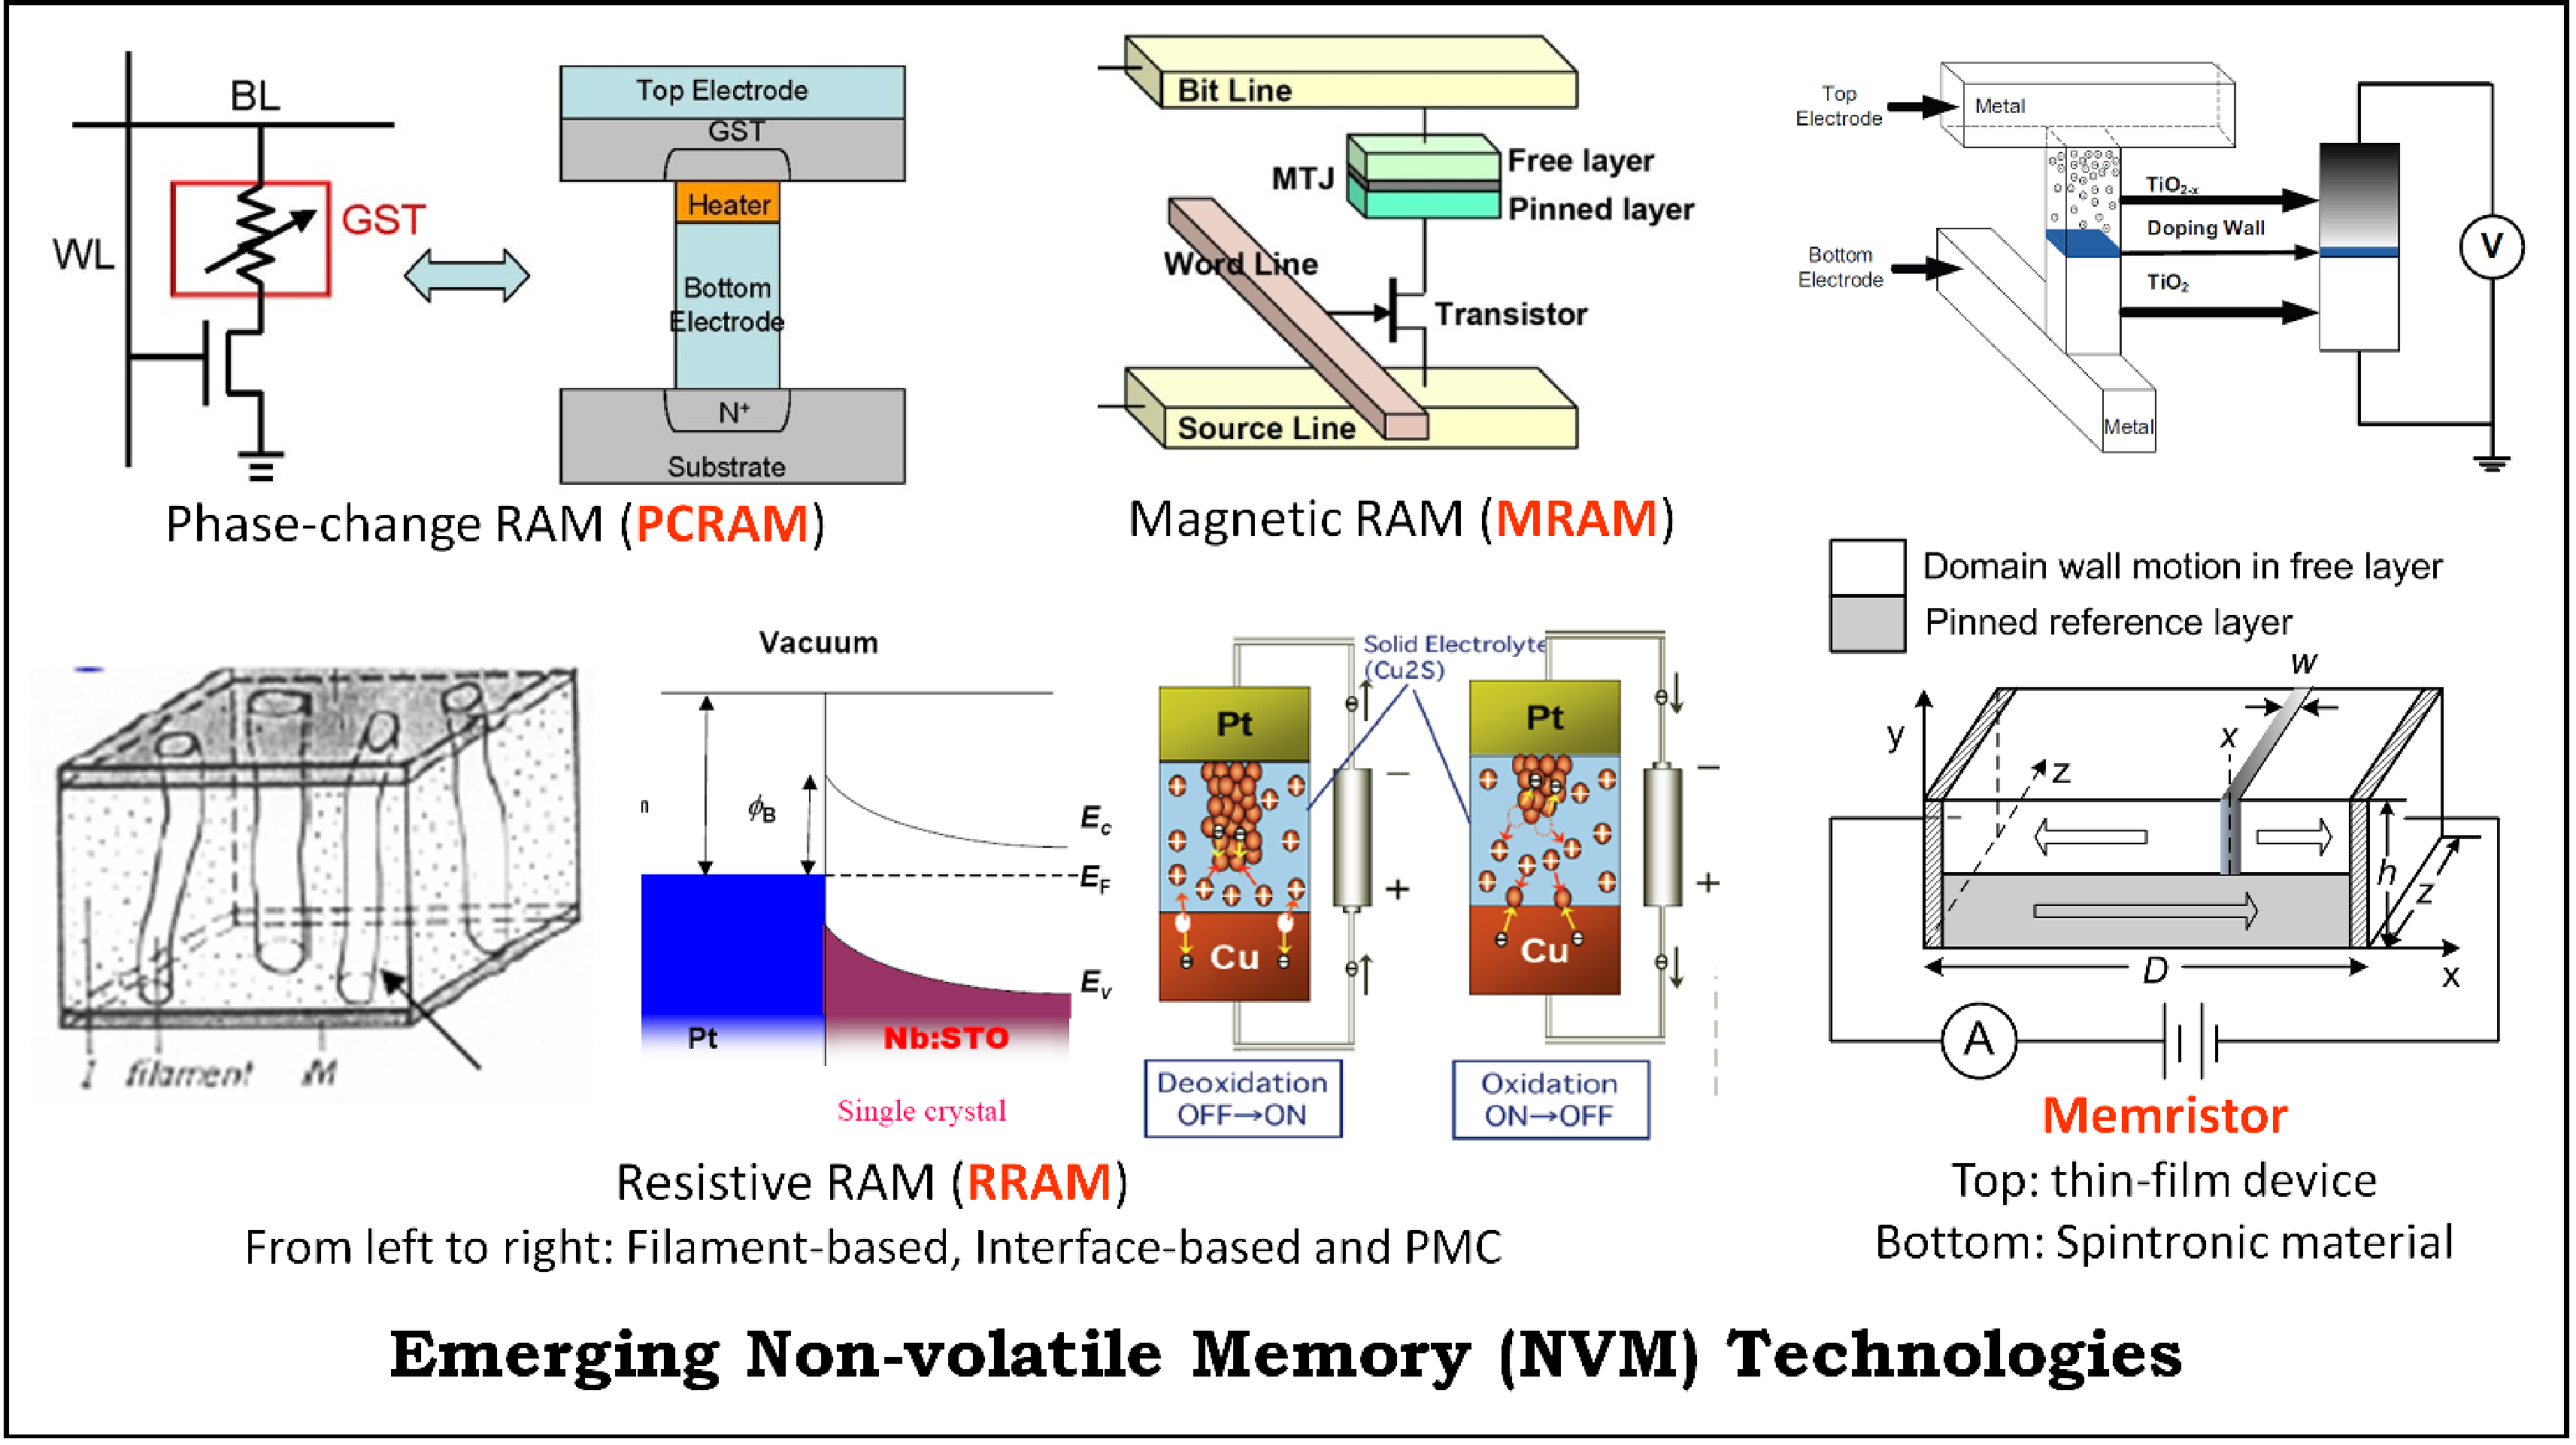
\includegraphics[width=0.95\textwidth]{./figure/1_technology_half.pdf}
\vspace{-10pt}
\caption{\textbf{Overview of Some Emerging Non-volatile Memory Technologies,} including Phase-Change RAM (PCRAM), Magnetic RAM (MRAM), resistive RAM (RRAM), and memristor. }
\label{technology}
\vspace{-10pt}
\end{figure}

\subsection{MRAM based on Spin-Torque Transfer RAM (STT-RAM)}
STT-RAM is a new type of Magnetic RAM (MRAM)~\cite{ITRS07,Hosomi05,MRAM:TTO+06,MRAM:ZBM+06,mram:ibm:maffitt}, which features non-volatility, fast writing/reading speed (\textless 10ns), high programming endurance (\textgreater 10$^{15}$cycles) and zero standby power~\cite{ITRS07}. The storage capability or programmability of MRAM arises from magnetic tunneling junction (MTJ), in which a thin tunneling dielectric, e.g., MgO., is sandwiched by two ferromagnetic layers, as shown in Figure~\ref{technology}. One ferromagnetic layer (``pinned layer'') is designed to have its magnetization pinned, while the magnetization of the other layer (``free layer'') can be flipped by a write event. An MTJ has a low (high) resistance if the magnetizations of the free layer and the pinned layer are parallel (anti-parallel). In first-generation MRAM design, the magnetization of free layer is changed by the current-induced magnetic field~\cite{Motoyoshi04,Ha04}. In STT-RAM, a new write mechanism called ``polarization-current-induced magnetization switching'' is introduced -- the magnetization of free layer is flipped by the electrical current directly. Because the current required to switch an MTJ resistance state is proportional to the MTJ cell area, STT-RAM is believed to have a better scaling property than the first-generation MRAM~\cite{Hosomi05,Kawahara07,MRAM:TTO+06,Diao07,Salahuddin07,Beach08,Kishi08}.

Continuous efforts on process development have been taken on yield improvement~\cite{Miura07}, write power reduction~\cite{Durlam03}, and high density~\cite{Lou08}. Prototyping STT-RAM chips have been demonstrated recently by various companies and research groups~\cite{Hosomi05,Kawahara07,Nebashi09,Motoyoshi04,Andre05,Kawahara08}. Commercial MRAM products have been launched by companies like Everspin (which is a spin-off from Freescale to expedite the technology commercialization in 2008) and NEC.

We have proposed a dynamic MTJ model with more accurate (transient) description for MTJ resistance switching~\cite{Chen08}. Compared to highly conceptual fixed resistance used in traditional STT-RAM design flow, the dynamic model can help to reduce 20\% pessimism in write time at TSMC $0.13{\mu}m$. The failure probability of STT-RAM cells due to parameter variations was considered and discussed in~\cite{Li09}. A model was proposed to predict memory yield and design optimization to minimize memory failures. MRAM potentially could be next-generation on-chip cache or memory due to its fast access and soft-error resistance. We will work toward this direction and look for new solutions and more applications to fast this procedure.

\subsection{Resistive RAM (RRAM)}
In an R-RAM cell, the data is stored as two (single-level cell, or SLC) or more resistance states (multi-level cell, or MLC) of the resistive switch device (RSD). Resistive switching in transition metal oxides was discovered in thin NiO film decades ago~\cite{Gibbons64}. From then, a large variety of metal-oxide materials have been verified to have resistive switching characteristics, including TiO$_2$~\cite{Fujimoto06}, NiO$_x$~\cite{Jung07}, Cr-doped SrTiO$_3$~\cite{Janousch07}, PCMO~\cite{Liu00}, and CMO~\cite{Hsu07} etc. Based on the storage mechanisms, RRAM materials can be cataloged as filament-based, interface-based, programmable-metallization-cell (PMC), etc. Based on the electrical property of resistive switching, RSDs can be divided into two categories: unipolar or bipolar.

Filament-based RRAM is a typical example of unipolar switching~\cite{Inoue} that has been widely investigated. The insulating material between two electrodes can be made conducting through a hopping or tunneling conduction path after the application of a sufficiently high voltage. %a process called electro-forming. 
The data storage could be achieved by break (RESET) or reconnect (SET) the conducting path. Programmable-metallization-cell (PMC)~\cite{Kozicki05} is a promising bipolar switching technology. The switching mechanism of PMC can be explained as forming or breaking the small metallic ``nanowire'' by moving the  metal ions between two sold metal electrodes.

\textbf{\underline{HL: Related work.}}

\subsection{Memristor}
Memristor, the fourth fundamental passive circuit element, was predicted by Professor Chua in 1971~\cite{Chua71}, based on the completeness of circuit theory. %Different from other electrical parameters resistance (\textit{R}), capacitance (\textit{C}) and inductance (\textit{L}), 
Memristance (\textit{M}) is a function of charge (\textit{q}),  which depends upon the historic behavior of the current (or voltage) profile~\cite{Chua76,Strukov08}. In 2008, 37 years after memristor was predicted in theory, the researchers at HP reported the first real device of a memristor. The memristive effect was achieved in a solid-state thin film two-terminal device by moving the doping front along the device as shown in Figure~\ref{technology}~\cite{Tour08}. Afterwards, magnetic technology provides the other possible methods to build a memristive system~\cite{Pershin08,Wang09}. Due to its unique historic characteristic, memristor has very broad application including nonvolatile memory, signal processing, control and learning system etc~\cite{Chen09}.

\textbf{\underline{HL: Related work.}} Indeed, HP Labs plan to unveil RRAM prototype chips based on memristor with crossbar arrays soon.

\begin{figure}
\centering
\vspace{-10pt}
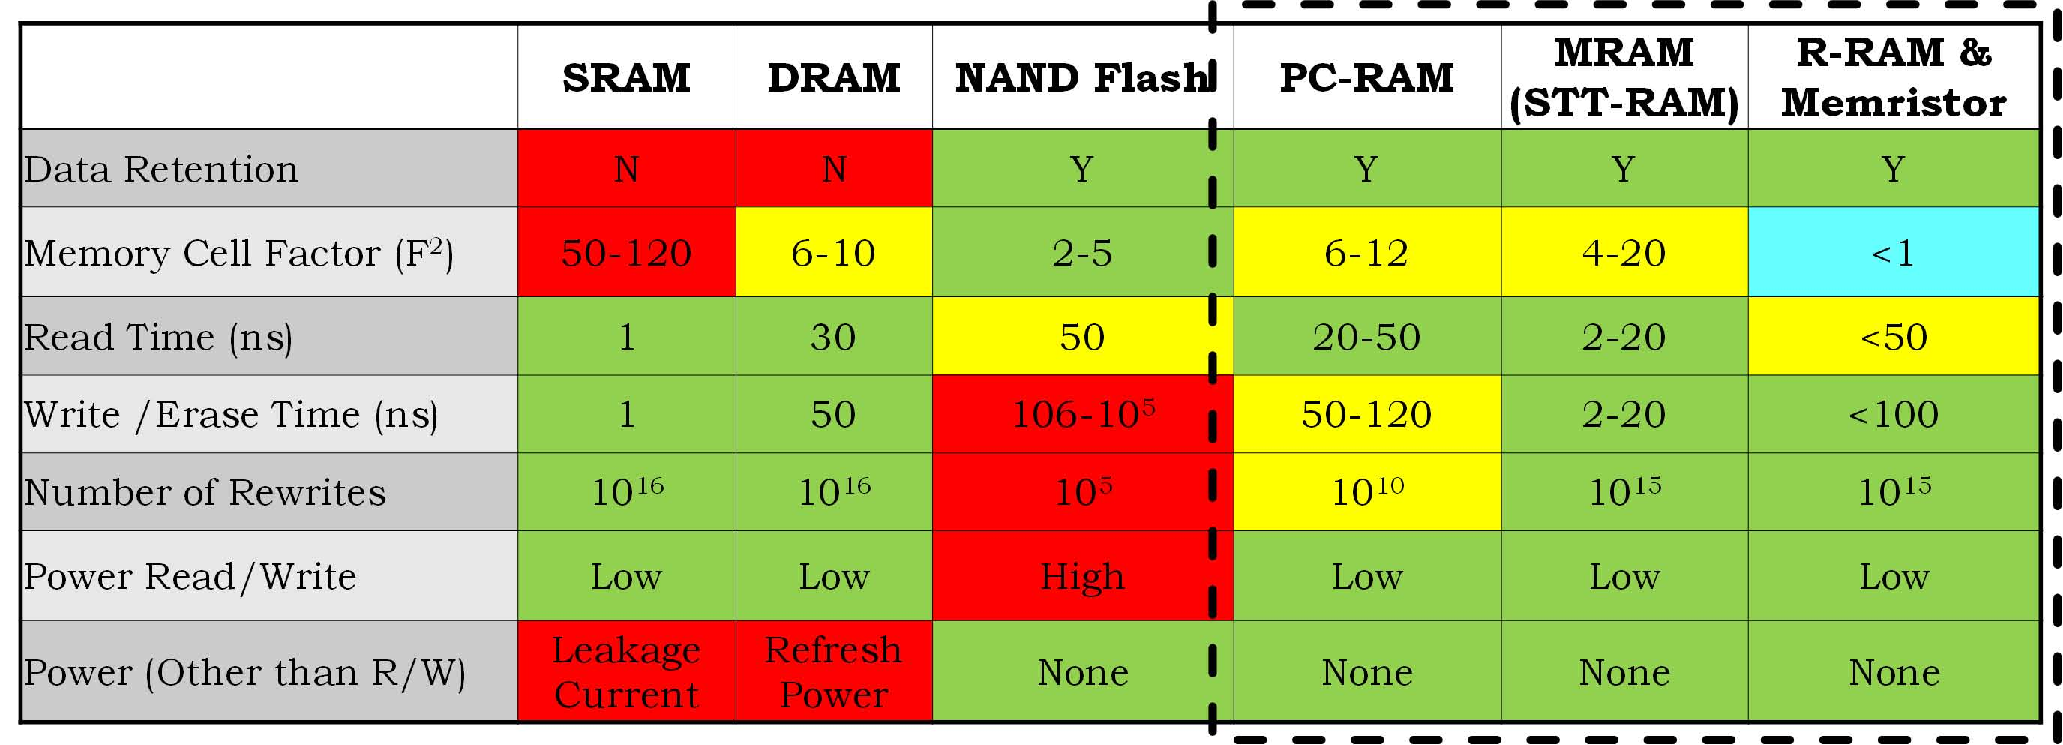
\includegraphics[width=0.9\textwidth]{./figure/2_table.pdf} 
\vspace{-10pt}
\caption{The comparison of various memory technologies~\cite{ITRS07}.}
\label{table}
\vspace{-10pt}
\end{figure}

\paragraph{Summary}
Figure~\ref{table} illustrates the comparison of emerging memory technologies -- PCRAM, MRAM (STT-RAM), RRAM and Memristor -- against the traditional main-stream SRAM, DRAM, and NAND-based Flash memory~\cite{ITRS07}. Note that both CMOS-compatible embedded MRAM (NEC)~\cite{MRAM:NEC09} and embedded PCRAM (Hitachi and STMicro)~\cite{Hanzawa07,PRAM:ST2004} have been demonstrated, paving the way of integrating these NVMs to the traditional memory hierarchies. In addition, the emerging 3D integration technologies~\cite{xie:jetcs06,Xie:dac08} enables cost-effective integration of these NVMs with CMOS logic circuits. With all the NVM technology advances in recent years, it is anticipated that the emerging NVM technologies will break important ground and move closer to market in the near future (``Non-volatile memory goes commercial", EEtimes, 12/02/2009).



\section{Proposed Research}
To enable the massive production and commercialization of the emerging non-volatile memories (NVMs), there are many critical technical issues to be solved. For example, how to integrate these new devices into the existing design flow? How to reduce the impacts of process variations? How to improve poor endurance and prolong life time? How to further increase memory capacity and throughput? etc. To answer these questions, we will start with the device modeling and analysis methodologies for the emerging NVM technologies; On top of it, novel circuit techniques will be proposed for each emerging memory technology based on its unique device characteristic. Our proposed research takes a holistic design perspective with close collaboration between two PIs with complementary expertise, aiming at accelerating the adoption of emerging NVMs for future computer architecture design.

%\subsection{Device Modeling and Design Flow}
\section{Task 1: Design Methodologies for Emerging Memory Technologies}

This proposed task focuses on device modeling and design flow and optimization
methodologies for memory design using emerging memory technologies.
%\textbf{\underline{HL: Need to be modified.}}
%To help the architectural level and system-level design of
%the SRAM-based or DRAM-based cache and memory, various
%modeling tools have been developed during the last decade. For
%example, CACTI~\cite{CACTI:NORM,PRAM:EVANS,PRAM:eCACTI,PRAM:CACTI60} and
%DRAMsim~\cite{DRAMsim} have become widely used in the
%computer architecture community to estimate the speed, power, and
%area parameters of SRAM and DRAM caches and main memory.
%Similarly, to explore new design opportunities that these emerging
%memory technologies can bring to the designers at architecture and
%system levels, it is imperative to have a high-level model
%for caches and memories built with emerging NVMs, such as MRAM/PCRAM.
%The model needs to provide the extraction of all important parameters, including access latency, dynamic access power, leakage power, die area, and I/O bandwidth \emph{etc.}, to facilitate architecture and system-level analysis and to bridge the gap between the abundant research activities at process and device levels and the lack of a high-level cache and memory model for emerging NVMs.




\subsection{Task 1.1: Device Modeling for Emerging Memory Technology}

Not like SRAM which is based on traditional CMOS technology, new materials are introduced in the emerging NVM technologies. For example, MRAM arises from magnetic tunneling junction (MTJ), and PCRAM technology is based on Ge$_2$--Sb$_2$--Te$_5$.
Due to the lack of knowledge on material physics of these NVM devices, most of research works on circuit, architecture and system levels nowadays are based on highly-simplified characteristics of the emerging devices. This methodology can cause a large design overhead, increase the production cost, and reduce the design margin, especially in the highly scaled technology with large process variations.  For example, the data storage element MTJ at a certain resistance state is usually modeled as a constant resistor by ignoring the dependency of the MTJ resistance on the magnitude of the read/write current driven by the NMOS selection transistor in an MRAM cell. Our previous work~\cite{Chen08} showed that after adopting a dynamic MTJ model that can take into account the time-varying electrical inputs in MRAM design flow, the design pessimism can be dramatically minimized and the memory array area can be reduced by more than 40\%. Therefore, one of the important tasks of our proposal is to build device models of the emerging NVM technologies for circuit design. Both dedicated device model and simplified behavioral model will be developed.

The dedicated device models, which will be built based on physical mechanism and corroborated by device measurements, need to satisfy three requirements: (1) These models should provide not only the accurate static characteristics (i.e., I-V relationship and high/low resistances), but also the reasonable dynamic behaviors, for example, what is the relationship between write current amplitude and write current pulse width and frequency in PCRAM design? How does MTJ resistance change during the magnetic direction transition of ferromagnetic layer? (2) The device parameter fluctuations induced by process variations, such as line-edge roughnesses (LERs), oxide thickness fluctuations (OTFs), and random discrete dopants (RDDs), will be also analyzed and integrated into the dedicated device model; and (3) the models should have reasonable runtime and be compatible to commercial EDA tools, i.e., HSPICE from Synopsys~\cite{synopsys} and Spectre from Cadence. Hence, Verilog-A or C language could be used to implement these models. The dedicated model will be used for memory optimization and timing/power analysis.

On top of it, the simplified behavioral models will be extracted. High-level languages, i.e. VHDL/Verilog or C will be used. The highly simplified conceptual model will be used for logic and functionality analysis.

\subsection{Task 1.2: Memory Circuit Design Flow}

\begin{wrapfigure}{r}{0.6\textwidth}\centering \centering   \includegraphics[width=0.6\textwidth]{./figure/HL-flow.pdf}
\caption{The proposed scope of device modeling and circuit analysis methodology for the emerging NVMs.}\label{flow}  \vspace{-20pt}
\end{wrapfigure}

Another important task of our proposal is to build a design environment that can be seamlessly integrated with the existing CMOS logic design flow. \textbf{\underline{HL: Modify figure}}. Figure~\ref{flow} illustrates the proposed scope of device modeling and circuit analysis methodology for the emerging NVMs. In Stage I, we will develop the dedicated device models be based on physical mechanism. On top of it, the simplified behavior models will be extracted. In Stage II, we will build an emerging memory design flow, which can realize the creation and optimization of novel hierarchal memory array structure and peripheral circuitry. The accuracy of the corresponding device model will determine the credibility of the design, such as critical timing/power simulation and corner analysis. Therefore, the dedicated device model will be used in this step. High-level synthesis and function verification will also be an important part in Stage II. The simplified conceptual model is expected to provide sufficient accuracy and %for logic and functionality analysis.
can be easily integrated in the commercial EDA tools and design methodologies such as \emph{Primetime} and \emph{Timemill} from Synopsys~\cite{synopsys} for more thoroughly analysis, \emph{i.e.}, the critical path timing at design corners. In Stage III, we will build IP's (Intelligence Properties) for emerging NVM technologies with the aid of the proposed design flow in Stage II. The IP's will provide the extracted parameters of memory array cell including area, dynamic and leakage power, access latency, \emph{etc.}, the recommendable memory array structures and the corresponding trade-offs, as well as the optimized peripheral circuitry design, \emph{i.e.}, sense amplifier and write drivers. Those IP's will be used in the researches at architectural and system levels.

The whole methodology and the corresponding outcomes, including device models, memory design flow, and IP's, will be distributed to the architecture and system design community. Our project will build a channel and provide a friendly interface among material development, device fabrication and architecture design.

%=========================================================================
%\textbf{I removed the Architectural modeling portion, since it is in 
%our other proposal, reviewers could easily compare and claim that we 
%duplicate the writing and decline both proposals.}

\begin{comment}
\subsubsection{Architectural Modeling}

Based on the device/circuit-level modeling and analysis methodologies described in Task 1-A, we will develop a PCRAM/MRAM simulator, which can be easily integrated with architecture simulators including Simplescalar-based single core simulator~\cite{simplescalar:computer02,sim-alpha}, and multi-core simulators such as M5~\cite{3D:M5},GEMS~\cite{martin:can05} or PTLsim~\cite{PTLsim}.

Note that tools such as CACTI~\cite{CACTI:NORM,PRAM:EVANS,PRAM:eCACTI,PRAM:CACTI60} and DRAMsim~\cite{DRAMsim} have been widely used in the computer architecture community to estimate the speed, power, and area parameters of the traditional caches and main memory. However, these existing tools were initiated and built based on the cache and memory modelings of SRAM/DRAM. The architectural modeling for PCRAM/MRAM raises unique research issues and challenges on building such simulators. First, some circuitry modules in PCRAM/MRAM have different requirements from those originally designed for SRAM/DRAM. For example, the existing sense amplifier model in CACTI~\cite{CACTI:NORM,PRAM:EVANS,PRAM:eCACTI,PRAM:CACTI60} and DRAMsim~\cite{DRAMsim} is voltage-mode sensing, while PCRAM data reading usually uses a current-mode sense amplifier. Second, due to the unique device mechanisms, the models of PCRAM/MRAM need specialized circuits to properly handle their operations. We can still take PCRAM as an example. The specific pulse shapes are required to heat up GST material quickly and to cool it down gradually during the RESET and especially SET operations. Hence, a model of the slow quench pulse shaper need to be created. Finally, the most obvious and important difference between PCRAM/MRAM and SRAM/DRAM is their distinct memory cell structure. PCRAM and MRAM typically use a simple ``1T1R'' (one-transistor-one-resistor) or ``1D1R'' (one-diode-one-resistor) structure, while SRAM and DRAM cell has a conventional ``6T'' structure and ``1T1C'' (one-transistor-one-capacitor) structure, respectively. The difference of cell structures directly leads to different cell sizes and array structures.

In addition, where to place these NVM memories in the traditional memory hierarchy also influences the modeling methodologies. For example, the emerging NVMs could be used as a replacement for on-chip cache or for off-chip DIMM (dual in-line memory module). Obviously, the performance/power of on-chip cache and off-chip DIMM would be quite different: When a NVM is integrated with logics on the same die, there is no off-chip pin limitation so that the interface between NVM and logic can be re-designed to provide a much higher bandwidth. Furthermore, off-chip memory is not affected by the thermal profile of the microprocessor core while the on-chip cache is affected by the heat dissipation from the hot cores. While higher on-chip temperature has a negative impact on SRAM/DRAM memory, it actually has a positive influence on PCRAM because the heat can facilitate the write operations of PCRAM cell. The performance estimation of PCRAM becomes much more complicated in such a case.
Moreover, building an accurate PCRAM/MRAM simulator needs close collaborations with the industry (see collaboration letters from HP, IBM, IMEC, and Seagate) to understand physics and circuit details, as well as architectural level requirements such as the interface/interconnect with the multi-core CPUs.

\end{comment}


\subsection{Task 1.3: Energy/Performance/Reliability Design Space Exploration}

The physical characters of a NVM cell is mainly depends
on the material characters and fabrication process. However, the circuit design
of the memory array, such as the access device of the memory cell, the operational
voltage, and the pheriphral circuitry, can also impact the operation
conditions of the cell, such as current and power consumption. In this task, we propose to explore the design space of the NVM memory array, and study the energy/performance/reliability tradeoffs for memory design with such emerging
memory technologies.  

Due to the intrinsic non-volatile characteristics of these emerging memory technology, naturally the read and write behaviors are asymmetric in terms of performance and energy. For example, the write-operation of PCRAM/MRAM requires a large current to be applied for a period of time so that the state of the storage junction is flipped; while the read-operation is realized by applying a small voltage to the cell and sensing the current across the cell.
We propose to analyze the constrained conditions of he design of NVM memory array, and study the sizing of the transistors as well as the operational voltages to investigate the tradeoff of the distinguishability~\footnote{During the read operation, the ratio of high resistance to low resistance in the storage junction reflects the distinguishability between logic 1 and 0}, energy consumption, lifetime and speed. For example, both the width of NMOS access device and word-line 
voltage can obviously affect the distinguishability. A higher word-line voltage or a larger NMOS device is more desirable to obtain a high distinguishability. However, the power consumption issues and area consideration always require a low voltage and small device size. 
Another example is on the lifetime/energy/performance tradeoff. 
For example, the lifetime of PCRAM is represented by the cycling
endurance, which is a function of pulse energy applied for 
the memory cell during the RESET writing. The reason for 
higher energy pulse induced cycle lifetime degradation 
is that the RESET resistance can be saturated when the 
writing current is higher than a critical level. This
"over programming`` phenomena can result in lager amorphous
volume, and then degrade the PCRAM��s lifetime. Consequently, 
a large write current can help improve the performance, but affect both lifetime and energy. Consequently, depending on the application,
we plan to investigate two optimization strategies: (1) \textit{Energy-driven optimization.} For low power application, such as mobile computing platform, energy consumption may be the most important design goals. We can optimize the word-line and bit-line voltage as well as the transistor sizing of the access NMOS device for memory array to achieve minimal energy consumption while satisfy constrains on lifetime, performance, and area. (2) \textit{Performance-driven optimization.} For high performance application, We can perform the optimization to achieve the best read/write performance while satisfy constrains on lifetime, energy, and area. Such optimization strategies can also be extended to lifetime-driven optimization and density-driven optimization.  


\subsection{Preliminary Result and Collaborations:}
The PI Li has built a combined magnetic and circuit design analysis and optimization methodology for MRAM, which has been proved to improve design efficiency significantly~\cite{Chen08} by test-chip design and fabrication at Seagate. We are also one of the first researchers to propose spintronic memristor structures~\cite{Wang09}, which was interviewed by IEEE Spectrum~\cite{Spectrum09}. The corresponding compact model and corner analysis~\cite{Chen09} have also been developed. In this project, we will further extend this methodology to other emerging NVMs, such as PCRAM.

The PSU PI Xie has developed a stacked SRAM cache
simulator called 3DCacti~\cite{xie:iccd05-3d, XIE:TVLSI2008-3DCacti},
which has been widely downloaded and used by other researchers.
The PI and co-PI have collaborated together when the PI Li was in Seagate,
to develop a preliminary version of MRAM simulator for cache stacking~\cite{Xie:dac08,XIE:HPCA09}.
Xie also collaborated with Dr. Norm Jouppi
from HP Labs, developed a preliminary version of PCRAM simulator~\cite{xie:pcramsim}.
We will extend our existing toolsets to support architectural exploration.
 

\input{circuit}
%\section{Task 3: Novel Applications}

\subsection{Memristor as novel sensing scheme}
The device structure for temperature sensor is in Fig. 3a. It consists of a long spin-valve strip which includes two ferromagnetic layers: reference layer and free layer. The magnetization direction of reference layer is fixed by coupling to a pinned magnetic reference layer. The free layer is divided by a domain-wall into two segments that have opposite magnetization directions to each other. The device time domain resistance depends upon domain wall position as:  , where  and  are the high and low resistance of the spin valve.   is the spin valve length and   is the domain wall position.

Domain wall velocity at finite temperature depends upon both spin torque excitation strength and thermal fluctuation magnitude. Fig. 4 shows the normalized domain wall velocity as a function of the normalized current density for different normalized thermal fluctuation magnitudes. Domain wall velocity increases as temperature increases. Temperature sensitive and insensitive regions can be observed. Curves with kneeling shapes are around critical current density, where the domain wall velocity is sensitive to thermal fluctuation magnitude. For temperature sensing, a biasing voltage pulse with constant magnitude is applied to the device.  Resistance difference before and after voltage pulse is measured. This resistance difference is calibrated to sense temperature. Higher temperature results a bigger resistance dropping as shown in Figure 5.

The temperature sensing memristor is operated at a region where its electric behavior is sensitive to temperature change. This is achieved through a combination of temperature dependent domain wall mobility and the positive feedback between resistance and driving strength in memristor. The positive feedback between resistance and driving strength is a unique property of the memrisor. Memristor's resistance depends upon the integration of current/voltage excitation. For a constant voltage pulse driving, higher temperature results an increased domain wall moving distance. The increased domain wall moving distance results a smaller resistance. The smaller resistance results a higher driving current density, thus providing positive feedback to further increase domain wall distance. This positive feedback accelerates domain wall speed and reduces device resistance further for a constant voltage pulse driving. Solid curves on the Fig. 5 are the resistance changes for the proposed spintronic memristor at different temperatures. Dash lines are the resistance dropping for a non-memristive device without positive feedback between resistance and the integration of driving strength.  The dash lines are equivalent to simulations with fixed driving current strength. It can be seen that positive feed back between resistance and driving strength in memristor significantly increases the temperature sensing margin.

\subsection{Reconfigurable System}

\subsection{: Hybrid system with other emerging devices.}





%
\section{Related Work}
\label{related}

In recently years, there have been active efforts on emerging NVM technologies. However, most of efforts were at process and device levels. Relatively, the architecture and system level analysis is less due to the lack of a high-level cache and memory model for emerging NVMs.

\paragraph{PCRAM.}
%%%% Device level
Compared to STT-RAM, PCM is even denser with an approximate cell area of $6\sim12F^2$~\cite{ITRS07}, where F is the feature size. In addition, phase change material has a key advantage of the excellent scalability within current CMOS fabrication methodology~\cite{Cho05,Kim06,Lai01,Pirovano03,Raoux08}.
Continue density improvement is the most important task for PCRAM process development. 2 and 4-bit MLC PCRAM material and the correponding write strategies were demonstrated by Nirshl et al.~\cite{Nirshl07}. New process integration techniques, such as ultra-small lithography independent contact area~\cite{Chen07-iedm} and unified 7.5nm dash-type confined cell~\cite{Im08}, could also help enhance density. Reliability is the major challenge in PCRAM process, which severely limits its applications. Researches on different angles have been done: Lacaita et al. discussed projected its impact on scaling ~\cite{Lacaita07}, Shih et al described the mechanisms of retention loss in GST material~\cite{Shih08}, and Lavizzari et al presented the impact of transient effects~\cite{Lavizzari08}. Accordingly, many device models were built from reliability~\cite{Ielmini07}, low-frequency noise~\cite{Fantini08}, statistical analysis~\cite{Mantegazza07} point of views. Those models mainly were dedicated to process and device, which cannot be borrowed by computer community.

%%%% circuit prototype to approve the potentials PCM
Many PCRAM prototypes have been demonstrated in the past years. In 2007, a 1.5V 512KB embedded PCRAM in a 0.13$\mu$m CMOS by Hitachi~\cite{Hanzawa07} and a 512b diode-switch PCRAM in a 90nm CMOS by Samsung~\cite{Lee07-isscc}. A year later, a 256Mb MLC PCRAM in a 90nm technology by STMicroelectronics~\cite{Bedeschi08}. Accordingly, a multi-level programming algorithm was developed and embedded into the chip, demonstrating 2b/cell feasibility. Very recently, a 45nm 1Gb 1.8V single-level cell (SLC) PCRAM was designed with 85ns random-access time and 9MB/s program throughput was demonstrated by Numonyx~\cite{Villa10}, and A 90nm 4Mb embedded PCRAM with 1.2V 12ns read access time and 1MB/s write throughput was made by STMicroelectronics~\cite{Sandre10}. In addition, The peripheral circuit design for high density diode-switch PCRAM was discussed in ISQED 2009~\cite{Li09}. Diode-switch PCRAM was demonstrated in VLSI Symposium 2007~\cite{Zhang07}

%%%% arch level for PCM

Discussions on endurance limitation were recently brought up to off-ship memories. Lee et al. proposed techniques to reduce the write accesses to PCM-based main memory to improve its endurance~\cite{ISCA09+MSPRAM}. One of the techniques utilizes the dirty bits in L2 at the word granularity to check if a word has been updated since it was last fetched on-chip. A technique along a similar line for PCM memory at bit level was proposed by Zhou et al.~\cite{ISCA09+Yang}. In this technique, a memory row is first read out, then compared with the new data, and finally written back for those changed values. This technique can significantly save performance and energy by avoiding pre-write operations. These technologies, however, all incurred significant access performance degradation and cannot be directly used in on-chip cache structure.


\paragraph{MRAM.}
%%% device
MRAM features non-volatility, fast access speed, zero standby power and high programming endurance\cite{Hosomi05,Diao07}. The research on MRAM material and device mainly devoted on spin-torque based MTJ due to its better performance, higher density, and better scalability compared to the conventional MRAM~\cite{Kawahara07,Salahuddin07,Beach08,Kishi08}. Certainly, the yield improvement is an important topic in nanoscale devices. Miura et al. presented a SPRAM with synthetic ferrimagnetic free layer, which has high immunity to read disturbance and sufficient margin between read and write currents~\cite{Miura07}. The MTJ structure with synthetic ferrimagnetic free layer can achieve a lower critical current density without degrading the thermal stability~\cite{Durlam03}.
Very recently, a 2-bit MLC (Multi-level cell) MTJ device was reported in~\cite{Lou08} for further density enhancement. Two-digit information -- $00$, $01$, $10$, and $11$, are represented by four MTJ resistance states. The transitions between different MTJ resistance states can be realized by passing the spin-polarized currents with different amplitudes and/or directions.

%%%% circuit prototype to approve the potentials
A 4Kb STT-RAM using tailored MTJ design was fabricated by Sony in $0.18{\mu}m$ technology in 2005~\cite{Hosomi05}. The test chip demonstrated that STT-RAM is a prominent candidate for the next generation memory because of its high speed, low power and high scalability. In 2007, Kawahara et al. prototyped a larger 2Mb STT-RAM in $0.2{\mu}m$ technology~\cite{Kawahara07}. This chip improves memory access latency by featuring an array scheme with bit-by-bit bidirectional current write and a prallelizing-direction current read. Recently, a even larger capacity -- 32Mb MRAM prototype in 90nm technology was demonstrated by NEC~\cite{Nebashi09}. A cell structure with 2 transistors and 1 magnetic tunneling junction (2T1MTJ) was adopted to improve access time to 12ns. Besides the SRAM-like array~\cite{Motoyoshi04,Andre05,Kawahara08}, other memory structures are also investigated by using MRAM/STT-RAM technology. In~\cite{Wang07}, Wang et. al. described a CAM structure based on conventional MRAM technology. In~\cite{Xu08}, Wu et. al. propsoed a novel STT-RAM read scheme with high sensing margin and illustrates a new CAM design. The possibility of applying STT-RAM in reconfigurable logic block for 3D-stacked reconfigurable spin processor was investigated~\cite{Sekikawa08}.

A write disturbance fault (WDF) model for conventional MRAM was proposed by Su et al.~\cite{Su08}. The fault affects the data stored in MRAM cells due to excessive magnetic filed during a write operation.
This should not be a problem to STT-RAM since it uses spin-polarized current to flip data. We have proposed a dynamic MTJ model with more accurate (transient) description for MTJ resistance switching~\cite{Chen08}. Compared to highly conceptual fixed resistance used in traditional STT-RAM design flow, the dynamic model can help to reduce 20\% pessimism in write time at TSMC $0.13{\mu}m$. The failure probability of STT-RAM cells due to parameter variations was considered and discussed in~\cite{Li09}. A model was proposed to predict memory yield and design optimization to minimize memory failures.

%%%% arch level for STT-RAM
At architecture level, there are several recent efforts in using STT-RAM as an on-chip last level cache. Desikan et. al. conducted an architectural evaluation of on-chip conventional MRAM cache in a single micro-processor~\cite{Desikan02}. Dong et al. developed a delay and energy model for MRAM-based cache and conducted a detailed comparison between the cache with SRAM and STT-RAM technologies in terms of area, performance and energy in the context of 3D stacking~\cite{MRAM:DONG08}. Sun et al. extended the application of STT-RAM based cache to Chip Multiprocessor (CMP) and proposed new techniques to improve latency and to reduce write energy~\cite{Sun09}.



\section{Broader Impacts, Outreach, and Education}

\paragraph{\textbf{Research Impact and Technical Merit:}}
Memory hierarchy design is one of the key components in modern computer
systems. The importance of the memory hierarchy
increases with the advances in performance of the
microprocessors~\cite{ITRS07}.  A key \textit{transformative aspect} of the proposed research is
that the success of the project will result in innovations in the computer architecture,
potentially leading to better performance, higher energy-efficient, and more reliable
computer systems.


\paragraph{\textbf{Collaborations and Partnership:}} It is naturally important to have industry support and guidance for this research.  The NYU-Poly PI Li has been with industry for 5 years before joining academia.  She has a strong connection with Memory
Product Group at Seagate, where she did research and led a design team on nonvolatile memories.    The PSU PI Xie worked for IBM Microelectronics division
before joining academia, and has built a good relationship with IBM
research. In the past 6 years as a faculty member, Xie has close collaborations with industry
partners. The proposed research has intrigued our industry partners, and the project will be
carried out with close collaboration with partners in several
companies, including IBM, Intel, HP, IMEC, Qualcomm, and Seagate.
%The industrial collaborators will
%play important roles in the proposed project by enabling the
%acquisition of realistic data, discussion of the practicality of
%ideas, placement of students in internships and permanent
%positions, and eventually the transfer of the technologies. By working
%closely with researchers in industry, the PIs will be able to ensure
%that the proposed methodologies and techniques are practical and have
%a real impact on industry.
The investigators
anticipate that the techniques and tools developed in this project will be
used in both classroom projects and academic/industrial
research. We will closely work with our industry partners to
transfer research results into commercial designs. The proposed
technology is of immense interest for companies.


\paragraph{\textbf{Outreach and Knowledge Dissemination:}} As part of outreach
efforts, the PIs will actively
disseminate results to a wide audience
and to different professional communities. The NYU-Poly PI Li believes that the communication between academia and industry
is very important. In NANOARCH 2009, she organized a panel on Emerging Technologies,
which brought industrial voices into emerging NVM research.
The PSU PI Xie has delivered over 30 invited talks in the
past at IEEE Chapters, universities, and companies.
He has been a tutorial speaker at several forums, offering
tutorials on 3D ICs in MICRO 2006, ISCA 2008, GLSVLSI 2008, and MICRO 2009~\cite{xie_url}.
Penn State is part of
the University-Industry-Government partnership called The
Technology Collaborative (TTC) that focuses on research, training
and education issues related with system design. The PI from Penn
State has been actively involved with their education programs and
have offered courses to the local industry in the past through
TTC. We will use this forum to disseminate findings of the
proposed research to industry practitioners, who in turn can
facilitate technology transition and incorporate research
breakthroughs in real systems.

\paragraph{\textbf{Women and Minority Student Recruiting Activities}}
While this research program will make contributions in educating all students to be well prepared for designing future computer systems, it will make additional efforts to promote diversity. Being a woman faculty herself, the NYU-Poly PI Li plans to actively recruit and mentor women and minority students. The PSU PI has an impressive record of graduate student advising, especially those from underrepresented groups, having graduated several women and minority graduate students. The PIs will continue to attract underrepresented students by getting their current graduate students from underrepresented communities to present their research at minority undergraduate institutions and to serve as role models. The PIs have been working with women and minority recruiting programs in both universities, i.e., the Multicultural Education and Programs at NYU-Poly and the WISER (Women in Science and Engineering Research) and MURE (Minority Undergraduate Research Experience) programs at PSU.


\paragraph{\textbf{Integration with Education:}} This project will
involve graduate and undergraduate students in all aspects of the
research. The PIs, as in the past, will actively integrate the
research results from this project into the graduate and
undergraduate curricula, especially related to computer architecture.
The NYU-Poly
PI teaches a graduate-level course EL5473 (Introduction to VLSI), and this
project will allow the PIs to integrate additional practical
material to make the class more appealing for engineering
students. A graduate-level course on advanced topics in computer architecture
will be developed at NYU-Poly in collaboration with colleagues who are
experts in architecture and circuit design. Undergraduate students
will be especially targeted and encouraged to pursue graduate
studies.  Support for undergraduate researchers will also be
sought from NSF REU supplements and  by involving
the outstanding students from the Schreyers Honors program at Penn
State.
Beyond involving students in all aspects of research, the PIs will
develop new courses on different aspects of advanced computer architecture and VLSI, to train the next generation work-force. In
addition, the PIs plans to organize workshops and tutorials at
major conferences to support other faculty to adapt new teaching
and research material in their curricula. Class notes, slides, and
laboratory manuals related to the new courses developed will be
made publicly available.
The PIs will educate industrial
practitioners and use this grant to disseminate findings to
industry practitioners, who in turn can facilitate technology
transition and incorporate research breakthroughs in real systems.


\paragraph{\textbf{Collaborative Teaching Experiments}:}  A graduate-level course
on emerging non-volatile memories will be simultaneously offered at Penn State and NYU-Poly (in a \textit{virtual classroom}) through an online course
delivery system (WebEx). Lectures will originate from both schools
based on the topics to be covered. The PIs will incorporate the
latest research outcomes from this project. Students at PSU and
NYU-Poly will also experiment with the tools developed as a part of
this research. This multi-institution education plan will not only
provide a unique opportunity for students to learn from experts in
other universities/areas but also promote collaborations among
students in different schools through working together on course
projects. Such remote collaboration is a critical skill in today's
global economy, where many companies have offices throughout the
world.

\paragraph{\textbf{Training of Students}:} Student mentoring is a key
component of this project. The PSU PI has excellent records in
student training.  His mentoring efforts were recently
  recognized with two Ph.D. students winning the department's ``Best Research Assisant Award" in 2008 and 2009. He has graduated 3 Ph.D. students (one in Sun
Microsystem, one in Qualcomm, and the other one in TSMC).
His students have received one best paper award (in ASPDAC
2008), and three best paper award nominations (in ICCAD 2006 and
ASPDAC 2009, 2010). The NYU-Poly PI just starts her academia career
recently in Fall 2009. She will be getting advice from the PSU PI on how to mentor and train graduate students during the course of this 3-year project.



\section{Project Management and Industry Collaborations}
%
%Please refer to the supplemental document titled Collaboration
%Plan.

The research team poses complementary skills required for the project. The PIs are well qualified for the proposed research with significant prior experience in various areas. The PI Prof. Li has 5-years industrial experience related to device modeling and circuit design with focus on emerging non-volatile memories, and just recently joined NYU-Poly as an assistant professor. The co-PI Prof. Xie's expertise span areas of VLSI and architecture, with extensive experience in architectures with emerging technologies, such as 3D architecture. The PIs will work in close coordination on different parts of this project. The integration of all these research components and tool will be a coordinated effort by all the investigators.

The project is a three-year effort involving multiple PhD students. Li will lead the effort in the first year with 2 PhD student from NYU with 1 PhD student from PSU on device modeling and build memory design flow in Task 1. From the second year, both PIs will work together with 1 PhD from each institute. While Xie continue exploring energy/performance/reliability design space in non-volatile memories, Li will focus on circuit techniques to improve NVM reliability with the aid of design flow built in first year. The yield and density enhancements will be the emphasis in the final year, which will be led by Xie.
Detailed project milestones are given in Figure~\ref{fig:plan}.

%\begin{comment}
%\begin{wrapfigure}{r}{0.5\textwidth}
%\vspace{-10pt}
\begin{figure}[htp]
\centering
% Requires \usepackage{graphicx}
%\epsfig{file=./figure/3DTESTDFT1.eps,width=0.7\textwidth}
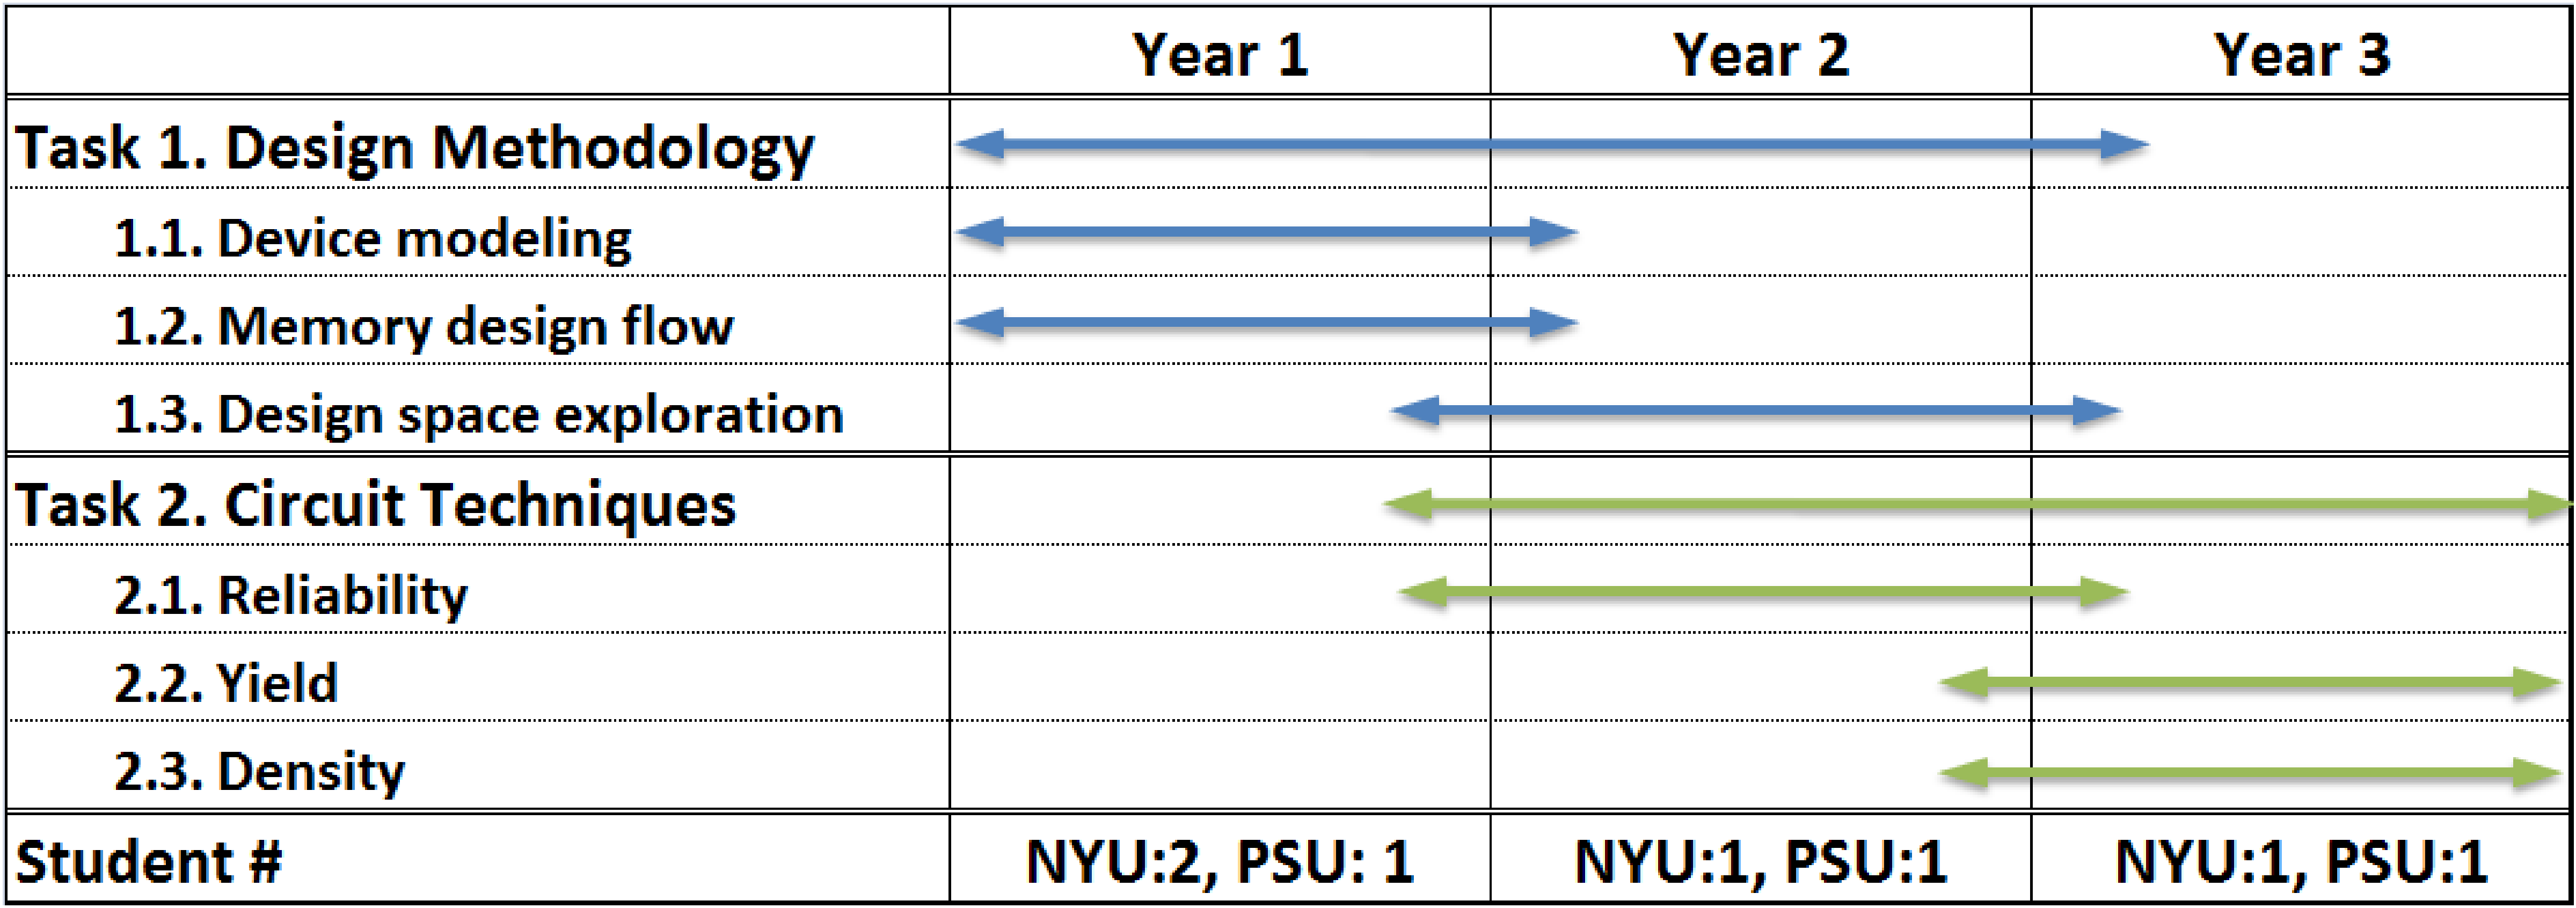
\includegraphics[width=0.6\textwidth]{./figure/schedule.pdf}
\vspace{-10pt} \caption{Project Management.} 
%(The first student in each task would be the lead).}
\label{fig:plan}
\end{figure}
%\vspace{-10pt}
%\end{wrapfigure}
%\end{comment}


The PIs have a well-established collaboration in the past years,
when the PI was still in Seagate,  and published preliminary results
on NVM architectures in DAC 2008 and HPCA 2009~\cite{XIE:HPCA09,Xie:dac08}. The existing collaboration
and preliminary results will allow rapid ramp-up for the proposed
research. The two teams will coordinate with each other via weekly
teleconferences and regular mutual visits (with only 4-hour driving between
two institutes).

\paragraph{\textbf{Industry Collaborations.}} By leveraging both PI's past industry experience and successful collaborations with companies, the project will be carried out in close collaboration with
industrial partners from IBM, HP, Intel, Qualcomm, Seagate, ITRI, as well as with
a partner from IMEC in Belgium.
The industrial collaborators will play important roles in the
proposed project by enabling the acquisition of realistic data,
discussion of the practicality of ideas, placement of students in
internships and permanent positions, and eventually the transfer of
the technologies. By working closely with researchers in industry,
the PIs will be able to ensure that the proposed methodologies and
tools are practical and have a real impact on industry.


\section{Results
from Prior NSF Support} \label{sec:prior}

\paragraph{Hai (Helen) Li} recently just joined NYU-Poly as an assistant
professor, after 5-years industrial experience in Qualcomm, Intel,
 and Seagate. She doesn't have any NSF grant yet.

\paragraph{\textbf{Yuan Xie:}} The most related prior NSF grant is
CCF-0903432 (ADAM: Architecture and Design Automation for 3D
Multi-core Systems; 08/2009-07/2012; \$480K). This project aims at
developing architectural design techniques and design automation
tools for future 3D multi-core architectures.
Xie actively collaborates with industry in 3D IC design research
(IBM, Qualcomm, Honda, and Seagate). He has published extensively in
the 3D IC design and 3D architecture areas, covering various aspects, including 3D
architecture~\cite{Xie:MTDT09,XIE:ASPDAC09-3D,XIE:HPCA09,Xie:dac08,xie:isca08,Xie:ISCA09,xie:isca06,xie:iccd05-3d,3D:LXB07,xie:tutorial-micro06} and
3D EDA
tools~\cite{XIE:ASPDAC2009-3Dcost,xie:iccd07-3d,XIE:ICCD08-3D,xie:isqed06-3d,xie:aspdac06,XIE:TVLSI2008-3DCacti,xie:iccd05-3d,xie:jetcs06}.

One of the benefits for 3D integration technologies is
the capability of enabling cost-effective heterogeneous integration, which
makes it much more practical to integrate emerging NVM with CMOS logic circuits.
Consequently, the research plan described in this proposal will
complement and be synergistic with the ongoing project.

The PIs have also submitted another proposal titled ``Collaborative Research:SHF:Small:Modeling, Architecture and Application for Emerging Memory Technologies'' to NSF-CISE-CCF-SHF program recently (December 2009), with a focused
scope of computer architecture research. The research topics work proposed in this proposal is circuit-oriented, and will complement and be synergistic with the other
pending proposal.

 \begin{comment}
\paragraph{Yuan Xie} has been awarded 7 NSF grants since 2003: 1) NSF
CNS 0454123:
 {\em SEAT -- Soft Error Analysis Toolset }(co-PI).
  06/2005-05/2008. This CRI (Computer Research Infrastructure)
  project aims at developing a soft error
  analysis toolset for hardware.
  Some of the results have been published
  \cite{xie:vlsid06-raj,
  xie:isvlsi06-soc,xie:selse06-raj,xie:selse06-balaji,xie:selse06-wang,
  xie:vlsid07-ser, xie:date07-timing, xie:date07-nbti, xie:isqed07-ser}.
2)NSF CAREER {\em CNS-0643902: Process Variation Aware Embedded
System Synthesis}.01/2007-12/2011. This CAREER project aims at
developing variation aware analysis and synthesis techniques for
embedded system design. The project has resulted in a few
publications~\cite{xie:date07-nbti,xie:date07-timing,xie:iccad07},
including ASP-DAC 2008 Best Paper Award
Nomination~\cite{xie:aspdac08}. 3)(NSF): {\em CCF 0702617: HoDoo:
Holistic Design of On-chip Interconnects}. 08/2007-07/2010. This
project aims at developing high performance, low power, reliable
on-chip network for future NoC architectures. 4)NSF {\em CNS
0720659: Hybrid Timing Analysis via Multi-mode Execution}.
01/2008-12/2010. This project aims at developing worst-case
execution time analysis techniques for embedded systems that
employ modern microarchitectures. He has been recently awarded 3
new NSF grants, which are all starting from 08/2009. These 3
grants include: 1) NSF 0903432. ``ADAM: Architecture and Design
Automation for 3D Multi-core Systems" (PI), 08/2009-07/2012. 2)NSF
0905365: ``Providing Predictable Timing for Task Migration in
Embedded Multi-Core Environments (TiME-ME)" (PI), 08/2009-07/2013.
3)NSF 0916887: ``Improving Lifetime Reliability for Reconfigurable
Embedded Systems" (Co-PI), 08/2009-07/2012.
\end{comment}



\pagebreak

%\setlength{\baselineskip}{13pt}
\setcounter{page}{1} \pagebreak
\begin{center}
{\Large  REFERENCES CITED} \\
\end{center}
\setlength{\itemsep}{0pt} \setlength{\parskip}{0pt}


%\bibliographystyle{plain}
\bibliographystyle{unsrt}

\bibliography{./bib/nsf-ihcs,./bib/se,./bib/hca,./bib/flash,./bib/lee-arch,./bib/helen,./bib/yuanxie,./bib/pram, ./bib/combined,./bib/thermal,./bib/3D-all,./bib/3D-1,./bib/vijay, ./bib/vijay-new,./bib/dram,./bib/vijay-2,./bib/mram,./bib/mram_1}
             

%\setlength{\baselineskip}{14pt}
%\pagebreak \setcounter{page}{1}
%\begin{center}
%{\Large BIOGRAPHICAL SKETCH} \\
%\end{center}
%\vspace{0.3in}
%\input{NSFbio-yuan}



\end{document}
